\documentclass[a4paper]{article}
% generated by Docutils <http://docutils.sourceforge.net/>
\usepackage{cmap} % fix search and cut-and-paste in Acrobat
\usepackage{ifthen}
\usepackage[T1]{fontenc}
\usepackage[utf8]{inputenc}
\usepackage{float} % float configuration
\floatplacement{figure}{H} % place figures here definitely
\usepackage{graphicx}
\usepackage{alltt}
\setcounter{secnumdepth}{0}
\usepackage{longtable,ltcaption,array}
\setlength{\extrarowheight}{2pt}
\newlength{\DUtablewidth} % internal use in tables

%%% Custom LaTeX preamble
% PDF Standard Fonts
\usepackage{mathptmx} % Times
\usepackage[scaled=.90]{helvet}
\usepackage{courier}

%%% User specified packages and stylesheets

%%% Fallback definitions for Docutils-specific commands

% hyperlinks:
\ifthenelse{\isundefined{\hypersetup}}{
  \usepackage[colorlinks=true,linkcolor=blue,urlcolor=blue]{hyperref}
  \usepackage{bookmark}
  \urlstyle{same} % normal text font (alternatives: tt, rm, sf)
}{}
\hypersetup{
  pdftitle={List of Optical Elements},
}

%%% Title Data
\title{\phantomsection%
  List of Optical Elements%
  \label{list-of-optical-elements}}
\author{}
\date{}

%%% Body
\begin{document}
\maketitle


\section{Summary of Effects in Optical Elements:%
  \label{summary-of-effects-in-optical-elements}%
}

\setlength{\DUtablewidth}{\linewidth}
\begin{longtable*}[c]{|p{0.181\DUtablewidth}|p{0.270\DUtablewidth}|p{0.262\DUtablewidth}|p{0.077\DUtablewidth}|p{0.165\DUtablewidth}|}
\hline
\textbf{%
element
} & \textbf{%
name
} & \textbf{%
class
} & \textbf{%
included
} & \textbf{%
z\_orders
} \\
\hline
\endfirsthead
\hline
\textbf{%
element
} & \textbf{%
name
} & \textbf{%
class
} & \textbf{%
included
} & \textbf{%
z\_orders
} \\
\hline
\endhead
\multicolumn{5}{c}{\hfill ... continued on next page} \\
\endfoot
\endlastfoot

armazones
 & 
armazones\_atmo\_default\_ter\_curve
 & 
AtmosphericTERCurve
 & 
True
 & 
{[}111{]}
 \\
\hline

armazones
 & 
armazones\_atmo\_dispersion
 & 
AtmosphericDispersion
 & 
True
 & 
{[}231{]}
 \\
\hline

armazones
 & 
armazones\_atmo\_skycalc\_ter\_curve
 & 
SkycalcTERCurve
 & 
False
 & 
{[}112{]}
 \\
\hline

ELT
 & 
scope\_surface\_list
 & 
SurfaceList
 & 
True
 & 
{[}20, 120{]}
 \\
\hline

ELT
 & 
scope\_vibration
 & 
Vibration
 & 
True
 & 
{[}244, 744{]}
 \\
\hline

ELT
 & 
eso\_combined\_reflection
 & 
TERCurve
 & 
False
 & 
{[}10, 110{]}
 \\
\hline

MICADO
 & 
micado\_static\_surfaces
 & 
SurfaceList
 & 
True
 & 
{[}20, 120{]}
 \\
\hline

MICADO
 & 
micado\_filter
 & 
FilterCurve
 & 
True
 & 
{[}114, 214{]}
 \\
\hline

MICADO
 & 
micado\_ncpas\_psf
 & 
NonCommonPathAberration
 & 
True
 & 
{[}241, 641{]}
 \\
\hline

micado\_detector\_array
 & 
full\_detector\_array
 & 
DetectorList
 & 
False
 & 
{[}90, 290, 390, 490{]}
 \\
\hline

micado\_detector\_array
 & 
detector\_window
 & 
DetectorList
 & 
True
 & 
{[}90, 290, 390, 490{]}
 \\
\hline

micado\_detector\_array
 & 
qe\_curve
 & 
QuantumEfficiencyCurve
 & 
True
 & 
{[}113{]}
 \\
\hline

micado\_detector\_array
 & 
exposure\_action
 & 
SummedExposure
 & 
True
 & 
{[}860{]}
 \\
\hline

micado\_detector\_array
 & 
dark\_current
 & 
DarkCurrent
 & 
True
 & 
{[}830{]}
 \\
\hline

micado\_detector\_array
 & 
detector\_linearity
 & 
LinearityCurve
 & 
True
 & 
{[}840{]}
 \\
\hline

micado\_detector\_array
 & 
shot\_noise
 & 
ShotNoise
 & 
True
 & 
{[}820{]}
 \\
\hline

micado\_detector\_array
 & 
readout\_noise
 & 
PoorMansHxRGReadoutNoise
 & 
True
 & 
{[}811{]}
 \\
\hline

default\_ro
 & 
relay\_psf
 & 
FieldConstantPSF
 & 
True
 & 
{[}262, 662{]}
 \\
\hline

default\_ro
 & 
relay\_surface\_list
 & 
SurfaceList
 & 
True
 & 
{[}20, 120{]}
 \\
\hline

MICADO\_IMG\_LR
 & 
micado\_wide\_field\_mirror\_list
 & 
SurfaceList
 & 
True
 & 
{[}20, 120{]}
 \\
\hline

MICADO\_IMG\_LR
 & 
micado\_adc\_3D\_shift
 & 
AtmosphericDispersionCorrection
 & 
True
 & 
{[}632, 232{]}
 \\
\hline
\end{longtable*}
\label{tbl-effects-summary}


\section{OpticalElement: \textquotedbl{}armazones\textquotedbl{}%
  \label{opticalelement-armazones}%
}

\textbf{Element}: atmosphere

\textbf{Alias}: ATMO

\textbf{Description}: Atmosphere and location details for Cerro Armazones


\subsection{Global properties%
  \label{global-properties}%
}

\begin{quote}
\begin{alltt}
    altitude : 3060
   longitude : -70.1918
    latitude : -24.5899
 temperature : 7
    humidity : 0.1
    pressure : 0.755
         pwv : 2.5
     airmass : !OBS.airmass
 pupil_angle : !OBS.pupil_angle
 pixel_scale : !INST.pixel_scale
element_name : armazones
\end{alltt}
\end{quote}


\subsection{Effects%
  \label{effects}%
}

Summary of Effects included in this optical element:

\setlength{\DUtablewidth}{\linewidth}
\begin{longtable*}[c]{|p{0.112\DUtablewidth}|p{0.358\DUtablewidth}|p{0.240\DUtablewidth}|p{0.101\DUtablewidth}|p{0.144\DUtablewidth}|}
\hline
\textbf{%
element
} & \textbf{%
name
} & \textbf{%
class
} & \textbf{%
included
} & \textbf{%
z\_orders {[}1{]}
} \\
\hline
\endfirsthead
\hline
\textbf{%
element
} & \textbf{%
name
} & \textbf{%
class
} & \textbf{%
included
} & \textbf{%
z\_orders {[}1{]}
} \\
\hline
\endhead
\multicolumn{5}{c}{\hfill ... continued on next page} \\
\endfoot
\endlastfoot

armazones
 & 
armazones\_atmo\_default\_ter\_curve
 & 
AtmosphericTERCurve
 & 
True
 & 
111
 \\
\hline

armazones
 & 
armazones\_atmo\_dispersion
 & 
AtmosphericDispersion
 & 
True
 & 
231
 \\
\hline

armazones
 & 
armazones\_atmo\_skycalc\_ter\_curve
 & 
SkycalcTERCurve
 & 
False
 & 
112
 \\
\hline
\end{longtable*}
\label{tbl-armazones}


\subsubsection{AtmosphericTERCurve: \textquotedbl{}armazones\_atmo\_default\_ter\_curve\textquotedbl{}%
  \label{atmospherictercurve-armazones-atmo-default-ter-curve}%
}

\textbf{Included by default}: \texttt{True}

\textbf{File Description}: atmospheric emission and transmission

\textbf{Class Description}: <no docstring>

\textbf{Changes}:

\begin{itemize}
\item 2019-07-24 (KL) Created file

\item 2019-08-09 (KL) Updated values for airmass 1.2, pwv 2.5
\end{itemize}


\paragraph{Data%
  \label{data}%
}


\paragraph{Meta-data%
  \label{meta-data}%
}

\begin{quote}
\begin{alltt}
       filename : TER_armazones_default_NIR_IMG.dat
           name : armazones_atmo_default_ter_curve
        include : True
       altitude : 3060
      longitude : -70.1918
       latitude : -24.5899
    temperature : 7
       humidity : 0.1
       pressure : 0.755
            pwv : 2.5
        airmass : !OBS.airmass
    pupil_angle : !OBS.pupil_angle
    pixel_scale : !INST.pixel_scale
   element_name : armazones
         author : Kieran Leschinski
         source : skycalc website for standard Armazones conditions
   date_created : 2019-07-24
  date_modified : 2019-08-09
         status : Design
           type : atmosphere:ter_curve
         season : entire year
           time : entire night
         action : transmission
wavelength_unit : um
  emission_unit : ph s-1 m-2 um-1 arcsec-2
        z_order : [111]
   ignore_wings : False
           area : !TEL.area
      area_unit : m2
       position : 0
\end{alltt}
\end{quote}


\subsubsection{AtmosphericDispersion: \textquotedbl{}armazones\_atmo\_dispersion\textquotedbl{}%
  \label{atmosphericdispersion-armazones-atmo-dispersion}%
}

\textbf{Included by default}: \texttt{True}

\textbf{File Description}: atmospheric dispersion

\textbf{Class Description}: Used to generate the wavelength bins based on shifts due to the atmosphere

\textbf{Changes}:

\begin{itemize}
\item \end{itemize}


\paragraph{Data%
  \label{id1}%
}


\paragraph{Meta-data%
  \label{id2}%
}

\begin{quote}
\begin{alltt}
          filename : None
              name : armazones_atmo_dispersion
          altitude : 3060
         longitude : -70.1918
          latitude : -24.5899
       temperature : 7
          humidity : 0.1
          pressure : 0.755
               pwv : 2.5
           airmass : !OBS.airmass
       pupil_angle : !OBS.pupil_angle
       pixel_scale : !INST.pixel_scale
      element_name : armazones
           z_order : [231]
           include : True
          wave_min : !SIM.spectral.wave_min
          wave_mid : !SIM.spectral.wave_mid
          wave_max : !SIM.spectral.wave_max
sub_pixel_fraction : !SIM.sub_pixel.fraction
         num_steps : 1000
\end{alltt}
\end{quote}


\subsubsection{SkycalcTERCurve: \textquotedbl{}armazones\_atmo\_skycalc\_ter\_curve\textquotedbl{}%
  \label{skycalctercurve-armazones-atmo-skycalc-ter-curve}%
}

\textbf{Included by default}: \texttt{False}

\textbf{File Description}: atmospheric spectra pulled from the skycalc server

\textbf{Class Description}: <no docstring>

\textbf{Changes}:

\begin{itemize}
\item \end{itemize}


\paragraph{Data%
  \label{id3}%
}


\paragraph{Meta-data%
  \label{id4}%
}

\begin{quote}
\begin{alltt}
    filename : None
        name : armazones_atmo_skycalc_ter_curve
     include : False
    altitude : 3060
   longitude : -70.1918
    latitude : -24.5899
 temperature : 7
    humidity : 0.1
    pressure : 0.755
         pwv : 2.5
     airmass : !OBS.airmass
 pupil_angle : !OBS.pupil_angle
 pixel_scale : !INST.pixel_scale
element_name : armazones
 observatory : armazones
        wmin : 699.9999999999999
        wmax : 2499.9999999999995
       wunit : um
      wdelta : 0.09999999999999999
     z_order : [112]
ignore_wings : False
      action : transmission
        area : !TEL.area
   area_unit : m2
    position : 0
\end{alltt}
\end{quote}


\section{OpticalElement: \textquotedbl{}ELT\textquotedbl{}%
  \label{opticalelement-elt}%
}

\textbf{Element}: telescope

\textbf{Alias}: TEL

\textbf{Description}: The extremely large telescope


\subsection{Global properties%
  \label{id5}%
}

\begin{quote}
\begin{alltt}
 temperature : !ATMO.temperature
element_name : ELT
\end{alltt}
\end{quote}


\subsection{Effects%
  \label{id6}%
}

Summary of Effects included in this optical element:

\setlength{\DUtablewidth}{\linewidth}
\begin{longtable*}[c]{|p{0.098\DUtablewidth}|p{0.284\DUtablewidth}|p{0.145\DUtablewidth}|p{0.110\DUtablewidth}|p{0.156\DUtablewidth}|}
\hline
\textbf{%
element
} & \textbf{%
name
} & \textbf{%
class
} & \textbf{%
included
} & \textbf{%
z\_orders {[}2{]}
} \\
\hline
\endfirsthead
\hline
\textbf{%
element
} & \textbf{%
name
} & \textbf{%
class
} & \textbf{%
included
} & \textbf{%
z\_orders {[}2{]}
} \\
\hline
\endhead
\multicolumn{5}{c}{\hfill ... continued on next page} \\
\endfoot
\endlastfoot

ELT
 & 
scope\_surface\_list
 & 
SurfaceList
 & 
True
 & 
20 .. 120
 \\
\hline

ELT
 & 
scope\_vibration
 & 
Vibration
 & 
True
 & 
244 .. 744
 \\
\hline

ELT
 & 
eso\_combined\_reflection
 & 
TERCurve
 & 
False
 & 
10 .. 110
 \\
\hline
\end{longtable*}
\label{tbl-elt}


\subsubsection{SurfaceList: \textquotedbl{}scope\_surface\_list\textquotedbl{}%
  \label{surfacelist-scope-surface-list}%
}

\textbf{Included by default}: \texttt{True}

\textbf{File Description}: list of ELT surfaces

\textbf{Class Description}: A Effect object containing a list of all surfaces in an optical element

\textbf{Changes}:

\begin{itemize}
\item 2018-11-19 (KL) Added meta data, added Action column

\item 2019-01-28 (KL) Fixed YAML format in meta data
\end{itemize}


\paragraph{Data%
  \label{id7}%
}
\leavevmode
\setlength{\DUtablewidth}{\linewidth}
\begin{longtable*}[c]{|p{0.063\DUtablewidth}|p{0.075\DUtablewidth}|p{0.075\DUtablewidth}|p{0.075\DUtablewidth}|p{0.145\DUtablewidth}|p{0.133\DUtablewidth}|p{0.342\DUtablewidth}|}
\hline
\textbf{%
name
} & \textbf{%
outer
} & \textbf{%
inner
} & \textbf{%
angle
} & \textbf{%
temperature
} & \textbf{%
action
} & \textbf{%
filename
} \\
\hline
\endfirsthead
\hline
\textbf{%
name
} & \textbf{%
outer
} & \textbf{%
inner
} & \textbf{%
angle
} & \textbf{%
temperature
} & \textbf{%
action
} & \textbf{%
filename
} \\
\hline
\endhead
\multicolumn{7}{c}{\hfill ... continued on next page} \\
\endfoot
\endlastfoot

M1
 & 
37.3
 & 
11.1
 & 
0.0
 & 
0.0
 & 
reflection
 & 
TER\_ELT\_mirror\_mgf2agal.dat
 \\
\hline

M2
 & 
4.2
 & 
0.545
 & 
0.0
 & 
0.0
 & 
reflection
 & 
TER\_ELT\_mirror\_mgf2agal.dat
 \\
\hline

M3
 & 
3.8
 & 
0.14
 & 
0.0
 & 
0.0
 & 
reflection
 & 
TER\_ELT\_mirror\_mgf2agal.dat
 \\
\hline

M4
 & 
2.4
 & 
0.0
 & 
7.75
 & 
0.0
 & 
reflection
 & 
TER\_ELT\_mirror\_aluminium.dat
 \\
\hline

M5
 & 
2.4
 & 
0.0
 & 
52.75
 & 
0.0
 & 
reflection
 & 
TER\_ELT\_mirror\_mgf2agal.dat
 \\
\hline
\end{longtable*}
\label{tbl-scope-surface-list}


\paragraph{Meta-data%
  \label{id8}%
}

\begin{quote}
\begin{alltt}
            filename : LIST_mirrors_ELT.tbl
                name : scope_surface_list
         temperature : !ATMO.temperature
        element_name : ELT
              author : Oliver Czoske
              source : None
        date_created : None
       date_modified : 2018-11-19
              status : Design - pre PDR list of ELT mirrors
                type : mirror:list
          outer_unit : m
          inner_unit : m
          angle_unit : degrees
    temperature_unit : deg_C
             z_order : [20, 120]
             include : True
  minimum_throughput : !SIM.spectral.minimum_throughput
            wave_min : !SIM.spectral.wave_min
            wave_max : !SIM.spectral.wave_max
report_table_include : True
\end{alltt}
\end{quote}


\subsubsection{Vibration: \textquotedbl{}scope\_vibration\textquotedbl{}%
  \label{vibration-scope-vibration}%
}

\textbf{Included by default}: \texttt{True}

\textbf{File Description}: residual vibration of telescope

\textbf{Class Description}: Creates a wavelength independent kernel image

\textbf{Changes}:

\begin{itemize}
\item \end{itemize}


\paragraph{Data%
  \label{id9}%
}


\paragraph{Meta-data%
  \label{id10}%
}

\begin{quote}
\begin{alltt}
        filename : None
            name : scope_vibration
     temperature : 7
    element_name : ELT
            fwhm : 0.001
     pixel_scale : 0.004
         z_order : [244, 744]
         include : True
   flux_accuracy : 0.001
  sub_pixel_flag : False
   convolve_mode : full
        wave_key : WAVE0
normalise_kernel : True
   width_n_fwhms : 4
\end{alltt}
\end{quote}


\subsubsection{TERCurve: \textquotedbl{}eso\_combined\_reflection\textquotedbl{}%
  \label{tercurve-eso-combined-reflection}%
}

\textbf{Included by default}: \texttt{False}

\textbf{File Description}: single combined reflection curve for clean ELT 5 mirror combination

\textbf{Class Description}: Transmission, Emissivity, Reflection Curve

\textbf{Changes}:

\begin{itemize}
\item 2019-11-06 (KL) Converted from .xlsx to .dat file, added ScopeSim meta data
\end{itemize}


\paragraph{Data%
  \label{id11}%
}


\paragraph{Meta-data%
  \label{id12}%
}

\begin{quote}
\begin{alltt}
     filename : TER_ELT_System_20190611.dat
         name : eso_combined_reflection
      include : False
  temperature : !ATMO.temperature
 element_name : ELT
       author : R. Holzloehner
       source : See ESO-306070 and ESO-293390 for background.
 date_created : 2018-09-18
date_modified : 2019-06-11
         type : TERCurve
       status : design
       action : reflection
        notes : ['Baseline coatings.', 'Fresh coatings without contamination.', '4nm roughness modeled.', 'Partly based on measured data by Tom Schneider (Gemini).', 'Reflection is for the combined M1-M5 system, not for individual mirrors']
      z_order : [10, 110]
 ignore_wings : False
\end{alltt}
\end{quote}


\section{OpticalElement: \textquotedbl{}MICADO\textquotedbl{}%
  \label{opticalelement-micado}%
}

\textbf{Element}: instrument

\textbf{Alias}: INST

\textbf{Description}: base configuration for MICADO


\subsection{Global properties%
  \label{id13}%
}

\begin{quote}
\begin{alltt}
 temperature : -190
element_name : MICADO
\end{alltt}
\end{quote}


\subsection{Effects%
  \label{id14}%
}

Summary of Effects included in this optical element:

\setlength{\DUtablewidth}{\linewidth}
\begin{longtable*}[c]{|p{0.098\DUtablewidth}|p{0.272\DUtablewidth}|p{0.284\DUtablewidth}|p{0.110\DUtablewidth}|p{0.156\DUtablewidth}|}
\hline
\textbf{%
element
} & \textbf{%
name
} & \textbf{%
class
} & \textbf{%
included
} & \textbf{%
z\_orders {[}2{]}
} \\
\hline
\endfirsthead
\hline
\textbf{%
element
} & \textbf{%
name
} & \textbf{%
class
} & \textbf{%
included
} & \textbf{%
z\_orders {[}2{]}
} \\
\hline
\endhead
\multicolumn{5}{c}{\hfill ... continued on next page} \\
\endfoot
\endlastfoot

MICADO
 & 
micado\_static\_surfaces
 & 
SurfaceList
 & 
True
 & 
20 .. 120
 \\
\hline

MICADO
 & 
micado\_filter
 & 
FilterCurve
 & 
True
 & 
114 .. 214
 \\
\hline

MICADO
 & 
micado\_ncpas\_psf
 & 
NonCommonPathAberration
 & 
True
 & 
241 .. 641
 \\
\hline
\end{longtable*}
\label{tbl-micado}


\subsubsection{SurfaceList: \textquotedbl{}micado\_static\_surfaces\textquotedbl{}%
  \label{surfacelist-micado-static-surfaces}%
}

\textbf{Included by default}: \texttt{True}

\textbf{File Description}: surfaces list for wide field optics

\textbf{Class Description}: A Effect object containing a list of all surfaces in an optical element

\textbf{Changes}:

\begin{itemize}
\item \{datetime.date(2019, 1, 28): '(KL) Changed column names and added units to header'\}

\item \{datetime.date(2019, 7, 10): '(KL) Shortened the list to only the swappable mirrors'\}
\end{itemize}


\paragraph{Data%
  \label{id15}%
}
\leavevmode
\setlength{\DUtablewidth}{\linewidth}
\begin{longtable*}[c]{|p{0.139\DUtablewidth}|p{0.072\DUtablewidth}|p{0.072\DUtablewidth}|p{0.072\DUtablewidth}|p{0.139\DUtablewidth}|p{0.151\DUtablewidth}|p{0.319\DUtablewidth}|}
\hline
\textbf{%
name
} & \textbf{%
outer
} & \textbf{%
inner
} & \textbf{%
angle
} & \textbf{%
temperature
} & \textbf{%
action
} & \textbf{%
filename
} \\
\hline
\endfirsthead
\hline
\textbf{%
name
} & \textbf{%
outer
} & \textbf{%
inner
} & \textbf{%
angle
} & \textbf{%
temperature
} & \textbf{%
action
} & \textbf{%
filename
} \\
\hline
\endhead
\multicolumn{7}{c}{\hfill ... continued on next page} \\
\endfoot
\endlastfoot

I00\_EntrWin
 & 
0.5
 & 
0.0
 & 
0
 & 
0
 & 
transmission
 & 
TER\_entrance\_window.dat
 \\
\hline

I01\_Fold1
 & 
0.5
 & 
0.0
 & 
45
 & 
-190
 & 
reflection
 & 
TER\_mirror\_gold.dat
 \\
\hline

I02\_Coli1
 & 
0.4
 & 
0.0
 & 
10
 & 
-190
 & 
reflection
 & 
TER\_mirror\_gold.dat
 \\
\hline

I03\_Coli2
 & 
0.2
 & 
0.0
 & 
10
 & 
-190
 & 
reflection
 & 
TER\_mirror\_gold.dat
 \\
\hline

I04\_Coli3
 & 
0.2
 & 
0.0
 & 
10
 & 
-190
 & 
reflection
 & 
TER\_mirror\_gold.dat
 \\
\hline

I05\_Fold2
 & 
0.2
 & 
0.0
 & 
45
 & 
-190
 & 
reflection
 & 
TER\_mirror\_gold.dat
 \\
\hline

I06\_Filter
 & 
0.2
 & 
0.0
 & 
0
 & 
-190
 & 
transmission
 & 
filters/TC\_filter\_blank.dat
 \\
\hline

I07\_ADC
 & 
0.2
 & 
0.0
 & 
0
 & 
-190
 & 
transmission
 & 
TER\_full\_adc.dat
 \\
\hline

I10\_Fold3
 & 
0.2
 & 
0.0
 & 
45
 & 
-190
 & 
reflection
 & 
TER\_mirror\_gold.dat
 \\
\hline

I11\_ReIm1
 & 
0.2
 & 
0.0
 & 
10
 & 
-190
 & 
reflection
 & 
TER\_mirror\_gold.dat
 \\
\hline

I12\_ReIm2
 & 
0.2
 & 
0.0
 & 
10
 & 
-190
 & 
reflection
 & 
TER\_mirror\_gold.dat
 \\
\hline

I13\_ReIm3
 & 
0.2
 & 
0.0
 & 
10
 & 
-190
 & 
reflection
 & 
TER\_mirror\_gold.dat
 \\
\hline
\end{longtable*}
\label{tbl-micado-static-surfaces}


\paragraph{Meta-data%
  \label{id16}%
}

\begin{quote}
\begin{alltt}
            filename : LIST_MICADO_mirrors_static.dat
                name : micado_static_surfaces
         temperature : -190
        element_name : MICADO
              author : Kieran Leschinski
              source : Ric's SPIE 2018 PPT presentation
        date_created : 2018-11-19
       date_modified : 2019-07-10
              status : Design - pre PDR list of all static MICADO surfaces
                type : mirror:list
               ETYPE : SURFLIST
                EDIM : 1
          outer_unit : m
          inner_unit : m
          angle_unit : degrees
    temperature_unit : deg_C
             z_order : [20, 120]
             include : True
  minimum_throughput : !SIM.spectral.minimum_throughput
            wave_min : !SIM.spectral.wave_min
            wave_max : !SIM.spectral.wave_max
report_table_include : True
\end{alltt}
\end{quote}


\subsubsection{FilterCurve: \textquotedbl{}micado\_filter\textquotedbl{}%
  \label{filtercurve-micado-filter}%
}

\textbf{Included by default}: \texttt{True}

\textbf{File Description}: transmission curve for filter

\textbf{Class Description}: kwargs

\textbf{Changes}:

\begin{itemize}
\item \end{itemize}


\paragraph{Data%
  \label{id17}%
}


\paragraph{Meta-data%
  \label{id18}%
}

\begin{quote}
\begin{alltt}
          filename : filters/TC_filter_Ks.dat
              name : micado_filter
       temperature : -190
      element_name : MICADO
       filter_name : !OBS.filter_name
   filename_format : filters/TC_filter_\{\}.dat
minimum_throughput : 0.000101
             outer : 0.2
        outer_unit : m
            author : Ric Davies
            source : Ric Davies
      date_created : 2017-11-20
     date_modified : 2017-11-20
            status : Design - pre PDR list of filters
              type : filter:transmission
            center : 2.144876984095012
             width : 0.3470169216021642
       blue_cutoff : 1.97136852329393
        red_cutoff : 2.3183854448960943
           z_order : [114, 214]
           include : True
      ignore_wings : False
            action : transmission
          position : -1
   wing_flux_level : None
\end{alltt}
\end{quote}


\subsubsection{NonCommonPathAberration: \textquotedbl{}micado\_ncpas\_psf\textquotedbl{}%
  \label{noncommonpathaberration-micado-ncpas-psf}%
}

\textbf{Included by default}: \texttt{True}

\textbf{File Description}: Effective NCPA induced PSF kernel

\textbf{Class Description}: Needed: pixel\_scale

\textbf{Changes}:

\begin{itemize}
\item 2018-11-19 (KL) updated meta data to new format
\end{itemize}


\paragraph{Data%
  \label{id19}%
}


\paragraph{Meta-data%
  \label{id20}%
}

\begin{quote}
\begin{alltt}
        filename : INST_MICADO_wavefront_error_budget.dat
            name : micado_ncpas_psf
     temperature : -190
    element_name : MICADO
     pixel_scale : 0.004
          author : Kieran Leschinski
         sources : Ric Davies email
    date_created : 2016-11-21
   date_modified : 2018-11-19
            type : instrument:wavefront_errors_list
          status : Idea - based on the WFE budget and emails with Ric
    wfe_rms_unit : nm
         z_order : [241, 641]
         include : True
   flux_accuracy : 0.001
  sub_pixel_flag : False
   convolve_mode : full
        wave_key : WAVE0
normalise_kernel : True
    kernel_width : None
    strehl_drift : 0.02
        wave_min : !SIM.spectral.wave_min
        wave_max : !SIM.spectral.wave_max
\end{alltt}
\end{quote}


\section{OpticalElement: \textquotedbl{}micado\_detector\_array\textquotedbl{}%
  \label{opticalelement-micado-detector-array}%
}

\textbf{Element}: detector

\textbf{Alias}: DET

\textbf{Description}: A set of 9 H4RG detectors


\subsection{Global properties%
  \label{id21}%
}

\begin{quote}
\begin{alltt}
image_plane_id : 0
   temperature : -230
           dit : !OBS.dit
          ndit : !OBS.ndit
  element_name : micado_detector_array
\end{alltt}
\end{quote}


\subsection{Effects%
  \label{id22}%
}

Summary of Effects included in this optical element:

\setlength{\DUtablewidth}{\linewidth}
\begin{longtable*}[c]{|p{0.218\DUtablewidth}|p{0.199\DUtablewidth}|p{0.247\DUtablewidth}|p{0.092\DUtablewidth}|p{0.199\DUtablewidth}|}
\hline
\textbf{%
element
} & \textbf{%
name
} & \textbf{%
class
} & \textbf{%
included
} & \textbf{%
z\_orders
} \\
\hline
\endfirsthead
\hline
\textbf{%
element
} & \textbf{%
name
} & \textbf{%
class
} & \textbf{%
included
} & \textbf{%
z\_orders
} \\
\hline
\endhead
\multicolumn{5}{c}{\hfill ... continued on next page} \\
\endfoot
\endlastfoot

micado\_detector\_array
 & 
full\_detector\_array
 & 
DetectorList
 & 
False
 & 
{[}90, 290, 390, 490{]}
 \\
\hline

micado\_detector\_array
 & 
detector\_window
 & 
DetectorList
 & 
True
 & 
{[}90, 290, 390, 490{]}
 \\
\hline

micado\_detector\_array
 & 
qe\_curve
 & 
QuantumEfficiencyCurve
 & 
True
 & 
{[}113{]}
 \\
\hline

micado\_detector\_array
 & 
exposure\_action
 & 
SummedExposure
 & 
True
 & 
{[}860{]}
 \\
\hline

micado\_detector\_array
 & 
dark\_current
 & 
DarkCurrent
 & 
True
 & 
{[}830{]}
 \\
\hline

micado\_detector\_array
 & 
detector\_linearity
 & 
LinearityCurve
 & 
True
 & 
{[}840{]}
 \\
\hline

micado\_detector\_array
 & 
shot\_noise
 & 
ShotNoise
 & 
True
 & 
{[}820{]}
 \\
\hline

micado\_detector\_array
 & 
readout\_noise
 & 
PoorMansHxRGReadoutNoise
 & 
True
 & 
{[}811{]}
 \\
\hline
\end{longtable*}
\label{tbl-micado-detector-array}


\subsubsection{DetectorList: \textquotedbl{}full\_detector\_array\textquotedbl{}%
  \label{detectorlist-full-detector-array}%
}

\textbf{Included by default}: \texttt{False}

\textbf{File Description}: MICADO detector array list

\textbf{Class Description}: A description of detector positions and properties

\textbf{Changes}:

\begin{itemize}
\item \{datetime.date(2017, 8, 12): '(OC) id changed to conform with spectroscopy report'\}

\item \{datetime.date(2018, 7, 26): '(OC) large gap (chips 5 and 6) reduced to 8 mm'\}

\item \{datetime.date(2018, 11, 19): '(KL) updated meta data to new format'\}

\item \{datetime.date(2019, 1, 28): '(KL) moved units into header'\}
\end{itemize}


\paragraph{Data%
  \label{id23}%
}

\begin{figure}
\noindent\makebox[\linewidth][c]{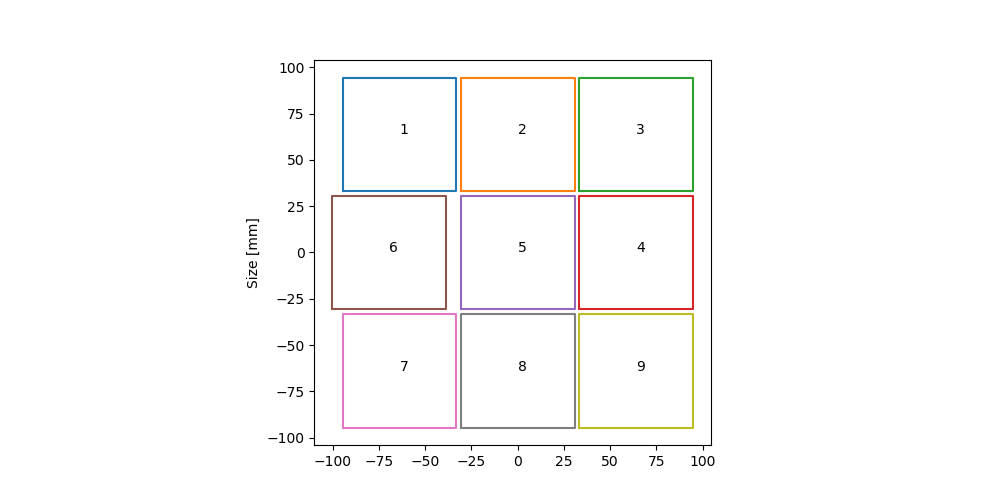
\includegraphics{full_detector_array.png}}\phantomsection\label{fig-full-detector-array}
\end{figure}

\setlength{\DUtablewidth}{\linewidth}
\begin{longtable*}[c]{|p{0.051\DUtablewidth}|p{0.086\DUtablewidth}|p{0.086\DUtablewidth}|p{0.086\DUtablewidth}|p{0.086\DUtablewidth}|p{0.075\DUtablewidth}|p{0.075\DUtablewidth}|p{0.133\DUtablewidth}|p{0.075\DUtablewidth}|p{0.063\DUtablewidth}|}
\hline
\textbf{%
id
} & \textbf{%
x\_cen
} & \textbf{%
y\_cen
} & \textbf{%
x\_size
} & \textbf{%
y\_size
} & \textbf{%
x\_len
} & \textbf{%
y\_len
} & \textbf{%
pixel\_size
} & \textbf{%
angle
} & \textbf{%
gain
} \\
\hline
\endfirsthead
\hline
\textbf{%
id
} & \textbf{%
x\_cen
} & \textbf{%
y\_cen
} & \textbf{%
x\_size
} & \textbf{%
y\_size
} & \textbf{%
x\_len
} & \textbf{%
y\_len
} & \textbf{%
pixel\_size
} & \textbf{%
angle
} & \textbf{%
gain
} \\
\hline
\endhead
\multicolumn{10}{c}{\hfill ... continued on next page} \\
\endfoot
\endlastfoot

1
 & 
-63.84
 & 
63.84
 & 
61.44
 & 
61.44
 & 
4096
 & 
4096
 & 
0.015
 & 
0.0
 & 
1.0
 \\
\hline

2
 & 
0.0
 & 
63.84
 & 
61.44
 & 
61.44
 & 
4096
 & 
4096
 & 
0.015
 & 
0.0
 & 
1.0
 \\
\hline

3
 & 
63.84
 & 
63.84
 & 
61.44
 & 
61.44
 & 
4096
 & 
4096
 & 
0.015
 & 
0.0
 & 
1.0
 \\
\hline

4
 & 
63.84
 & 
0.0
 & 
61.44
 & 
61.44
 & 
4096
 & 
4096
 & 
0.015
 & 
0.0
 & 
1.0
 \\
\hline

5
 & 
0.0
 & 
0.0
 & 
61.44
 & 
61.44
 & 
4096
 & 
4096
 & 
0.015
 & 
0.0
 & 
1.0
 \\
\hline

6
 & 
-69.44
 & 
0.0
 & 
61.44
 & 
61.44
 & 
4096
 & 
4096
 & 
0.015
 & 
0.0
 & 
1.0
 \\
\hline

7
 & 
-63.84
 & 
-63.84
 & 
61.44
 & 
61.44
 & 
4096
 & 
4096
 & 
0.015
 & 
0.0
 & 
1.0
 \\
\hline

8
 & 
0.0
 & 
-63.84
 & 
61.44
 & 
61.44
 & 
4096
 & 
4096
 & 
0.015
 & 
0.0
 & 
1.0
 \\
\hline

9
 & 
63.84
 & 
-63.84
 & 
61.44
 & 
61.44
 & 
4096
 & 
4096
 & 
0.015
 & 
0.0
 & 
1.0
 \\
\hline
\end{longtable*}
\label{tbl-full-detector-array}


\paragraph{Meta-data%
  \label{id24}%
}

\begin{quote}
\begin{alltt}
            filename : FPA_array_layout.dat
                name : full_detector_array
             include : False
      image_plane_id : 0
         temperature : -230
                 dit : !OBS.dit
                ndit : !OBS.ndit
        element_name : micado_detector_array
    active_detectors : all
              author : Oliver Czoske
             sources : E-MCD-FPA-572089EB.uda, ELT-TRE-MCD-56300-0011
        date_created : 2017-06-28
       date_modified : 2018-07-26
                type : detector:chip_list
          x_cen_unit : mm
          y_cen_unit : mm
            xhw_unit : mm
            yhw_unit : mm
          x_len_unit : pix
          y_len_unit : pix
        pixsize_unit : mm
          angle_unit : deg
           gain_unit : electron/adu
             z_order : [90, 290, 390, 490]
         pixel_scale : !INST.pixel_scale
 report_plot_include : True
report_table_include : True
         x_size_unit : mm
         y_size_unit : mm
\end{alltt}
\end{quote}


\subsubsection{DetectorList: \textquotedbl{}detector\_window\textquotedbl{}%
  \label{detectorlist-detector-window}%
}

\textbf{Included by default}: \texttt{True}

\textbf{File Description}:

\textbf{Class Description}: A description of detector positions and properties

\textbf{Changes}:

\begin{itemize}
\item \end{itemize}


\paragraph{Data%
  \label{id25}%
}

\begin{figure}
\noindent\makebox[\linewidth][c]{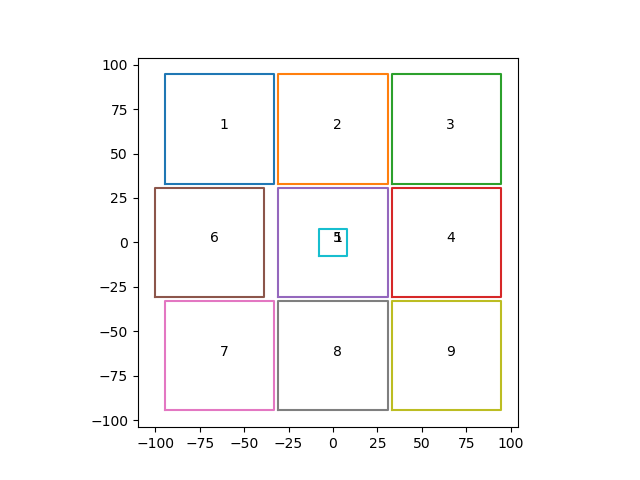
\includegraphics{detector_window.png}}\phantomsection\label{fig-detector-window}
\end{figure}

\setlength{\DUtablewidth}{\linewidth}
\begin{longtable*}[c]{|p{0.051\DUtablewidth}|p{0.133\DUtablewidth}|p{0.075\DUtablewidth}|p{0.063\DUtablewidth}|p{0.075\DUtablewidth}|p{0.075\DUtablewidth}|p{0.086\DUtablewidth}|p{0.086\DUtablewidth}|}
\hline
\textbf{%
id
} & \textbf{%
pixel\_size
} & \textbf{%
angle
} & \textbf{%
gain
} & \textbf{%
x\_cen
} & \textbf{%
y\_cen
} & \textbf{%
x\_size
} & \textbf{%
y\_size
} \\
\hline
\endfirsthead
\hline
\textbf{%
id
} & \textbf{%
pixel\_size
} & \textbf{%
angle
} & \textbf{%
gain
} & \textbf{%
x\_cen
} & \textbf{%
y\_cen
} & \textbf{%
x\_size
} & \textbf{%
y\_size
} \\
\hline
\endhead
\multicolumn{8}{c}{\hfill ... continued on next page} \\
\endfoot
\endlastfoot

1
 & 
0.015
 & 
0.0
 & 
1.0
 & 
0.0
 & 
0.0
 & 
15.36
 & 
15.36
 \\
\hline
\end{longtable*}
\label{tbl-detector-window}


\paragraph{Meta-data%
  \label{id26}%
}

\begin{quote}
\begin{alltt}
            filename : None
                name : detector_window
             include : True
      image_plane_id : 0
         temperature : -230
                 dit : !OBS.dit
                ndit : !OBS.ndit
        element_name : micado_detector_array
          x_cen_unit : mm
          y_cen_unit : mm
            xhw_unit : mm
            yhw_unit : mm
        pixsize_unit : mm
          angle_unit : deg
           gain_unit : electron/adu
             z_order : [90, 290, 390, 490]
          array_dict : \{'id': [1], 'pixsize': [0.015], 'angle': [0.0], 'gain': [1.0], 'x_cen': [0.0], 'y_cen': [0.0], 'xhw': [7.68], 'yhw': [7.68]\}
         pixel_scale : !INST.pixel_scale
    active_detectors : all
 report_plot_include : True
report_table_include : True
         x_size_unit : mm
         y_size_unit : mm
\end{alltt}
\end{quote}


\subsubsection{QuantumEfficiencyCurve: \textquotedbl{}qe\_curve\textquotedbl{}%
  \label{quantumefficiencycurve-qe-curve}%
}

\textbf{Included by default}: \texttt{True}

\textbf{File Description}: Quantum efficiency curves for each detector

\textbf{Class Description}: <no docstring>

\textbf{Changes}:

\begin{itemize}
\item \{datetime.date(2018, 11, 19): '(KL) updated meta data to new format'\}

\item \{datetime.date(2019, 8, 9): '(KL) Added action keyword to meta data'\}
\end{itemize}


\paragraph{Data%
  \label{id27}%
}


\paragraph{Meta-data%
  \label{id28}%
}

\begin{quote}
\begin{alltt}
       filename : QE_detector_H2RG.dat
           name : qe_curve
 image_plane_id : 0
    temperature : -230
            dit : !OBS.dit
           ndit : !OBS.ndit
   element_name : micado_detector_array
         author : Kieran Leschinski
        sources : Finger+ 2008 SPIE
   date_created : 2016-01-01
  date_modified : 2019-08-09
           type : detector:quantum_efficiency
         status : Design - guestimated by reading off the graph in Finger+ 2008
wavelength_unit : um
         action : transmission
        z_order : [113]
        include : True
   ignore_wings : False
       position : -1
\end{alltt}
\end{quote}


\subsubsection{SummedExposure: \textquotedbl{}exposure\_action\textquotedbl{}%
  \label{summedexposure-exposure-action}%
}

\textbf{Included by default}: \texttt{True}

\textbf{File Description}: Summing up sky signal for all DITs and NDITs

\textbf{Class Description}: <no docstring>

\textbf{Changes}:

\begin{itemize}
\item \end{itemize}


\paragraph{Data%
  \label{id29}%
}


\paragraph{Meta-data%
  \label{id30}%
}

\begin{quote}
\begin{alltt}
      filename : None
          name : exposure_action
image_plane_id : 0
   temperature : -230
           dit : !OBS.dit
          ndit : !OBS.ndit
  element_name : micado_detector_array
       z_order : [860]
       include : True
\end{alltt}
\end{quote}


\subsubsection{DarkCurrent: \textquotedbl{}dark\_current\textquotedbl{}%
  \label{darkcurrent-dark-current}%
}

\textbf{Included by default}: \texttt{True}

\textbf{File Description}: MICADO dark current

\textbf{Class Description}: required: dit, ndit, value

\textbf{Changes}:

\begin{itemize}
\item \end{itemize}


\paragraph{Data%
  \label{id31}%
}


\paragraph{Meta-data%
  \label{id32}%
}

\begin{quote}
\begin{alltt}
      filename : None
          name : dark_current
image_plane_id : 0
   temperature : -230
           dit : !OBS.dit
          ndit : !OBS.ndit
  element_name : micado_detector_array
         value : 0.1
       z_order : [830]
       include : True
\end{alltt}
\end{quote}


\subsubsection{LinearityCurve: \textquotedbl{}detector\_linearity\textquotedbl{}%
  \label{linearitycurve-detector-linearity}%
}

\textbf{Included by default}: \texttt{True}

\textbf{File Description}: Linearity characteristics of H4RG chips

\textbf{Class Description}: <no docstring>

\textbf{Changes}:

\begin{itemize}
\item 2018-11-19 (KL) updated meta data to new format

\item 2019-08-14 (KL) replaced long 1000000000 with 1e99
\end{itemize}


\paragraph{Data%
  \label{id33}%
}


\paragraph{Meta-data%
  \label{id34}%
}

\begin{quote}
\begin{alltt}
      filename : FPA_linearity.dat
          name : detector_linearity
image_plane_id : 0
   temperature : -230
           dit : !OBS.dit
          ndit : !OBS.ndit
  element_name : micado_detector_array
        author : Kieran Leschinski
       sources : Ingraham+ 2014 - Gemini Calibrations II for H2RG
  date_created : 2016-01-01
 date_modified : 2018-11-19
          type : detector:linearity
        status : Design - approximated from the H2RG
 incident_unit : ph
 measured_unit : ph
       z_order : [840]
       include : True
\end{alltt}
\end{quote}


\subsubsection{ShotNoise: \textquotedbl{}shot\_noise\textquotedbl{}%
  \label{shotnoise-shot-noise}%
}

\textbf{Included by default}: \texttt{True}

\textbf{File Description}: apply poisson shot noise to images

\textbf{Class Description}: <no docstring>

\textbf{Changes}:

\begin{itemize}
\item \end{itemize}


\paragraph{Data%
  \label{id35}%
}


\paragraph{Meta-data%
  \label{id36}%
}

\begin{quote}
\begin{alltt}
      filename : None
          name : shot_noise
image_plane_id : 0
   temperature : -230
           dit : !OBS.dit
          ndit : !OBS.ndit
  element_name : micado_detector_array
       z_order : [820]
       include : True
   random_seed : !SIM.random.seed
\end{alltt}
\end{quote}


\subsubsection{PoorMansHxRGReadoutNoise: \textquotedbl{}readout\_noise\textquotedbl{}%
  \label{poormanshxrgreadoutnoise-readout-noise}%
}

\textbf{Included by default}: \texttt{True}

\textbf{File Description}: Readout noise frames

\textbf{Class Description}: <no docstring>

\textbf{Changes}:

\begin{itemize}
\item \end{itemize}


\paragraph{Data%
  \label{id37}%
}


\paragraph{Meta-data%
  \label{id38}%
}

\begin{quote}
\begin{alltt}
         filename : None
             name : readout_noise
   image_plane_id : 0
      temperature : -230
              dit : !OBS.dit
             ndit : !OBS.ndit
     element_name : micado_detector_array
        noise_std : 12
       n_channels : 64
          z_order : [811]
          include : True
pedestal_fraction : 0.3
    read_fraction : 0.4
    line_fraction : 0.25
 channel_fraction : 0.05
      random_seed : !SIM.random.seed
\end{alltt}
\end{quote}


\section{OpticalElement: \textquotedbl{}default\_ro\textquotedbl{}%
  \label{opticalelement-default-ro}%
}

\textbf{Element}: relay\_optics

\textbf{Alias}: RO

\textbf{Description}: Simple stand-alone relay optics module


\subsection{Global properties%
  \label{id39}%
}

\begin{quote}
\begin{alltt}
 temperature : !ATMO.temperature
element_name : default_ro
\end{alltt}
\end{quote}


\subsection{Effects%
  \label{id40}%
}

Summary of Effects included in this optical element:

\setlength{\DUtablewidth}{\linewidth}
\begin{longtable*}[c]{|p{0.133\DUtablewidth}|p{0.226\DUtablewidth}|p{0.203\DUtablewidth}|p{0.110\DUtablewidth}|p{0.156\DUtablewidth}|}
\hline
\textbf{%
element
} & \textbf{%
name
} & \textbf{%
class
} & \textbf{%
included
} & \textbf{%
z\_orders {[}2{]}
} \\
\hline
\endfirsthead
\hline
\textbf{%
element
} & \textbf{%
name
} & \textbf{%
class
} & \textbf{%
included
} & \textbf{%
z\_orders {[}2{]}
} \\
\hline
\endhead
\multicolumn{5}{c}{\hfill ... continued on next page} \\
\endfoot
\endlastfoot

default\_ro
 & 
relay\_psf
 & 
FieldConstantPSF
 & 
True
 & 
262 .. 662
 \\
\hline

default\_ro
 & 
relay\_surface\_list
 & 
SurfaceList
 & 
True
 & 
20 .. 120
 \\
\hline
\end{longtable*}
\label{tbl-default-ro}


\subsubsection{FieldConstantPSF: \textquotedbl{}relay\_psf\textquotedbl{}%
  \label{fieldconstantpsf-relay-psf}%
}

\textbf{Included by default}: \texttt{True}

\textbf{File Description}: SCAO PSF

\textbf{Class Description}: <no docstring>

\textbf{Changes}:

\begin{itemize}
\item \end{itemize}


\paragraph{Data%
  \label{id41}%
}


\paragraph{Meta-data%
  \label{id42}%
}

\begin{quote}
\begin{alltt}
        filename : PSF_SCAO_ConstPSF_0_5off.fits
            name : relay_psf
     temperature : 7
    element_name : default_ro
         warning : Default PSF is NOT field varying. See documentation.
          SIMPLE : True
          BITPIX : 8
           NAXIS : 0
          EXTEND : True
          AUTHOR : Kieran Leschinski
        DATE_CRE : 2019-07-30
        DATE_MOD : 2019-07-30
          SOURCE : AnisoCADO
          STATUS : Best guess for a standard observations
           ETYPE : CONSTPSF
            ECAT : -1
           EDATA : 1
         XOFFSET : 0
         YOFFSET : 5
         z_order : [262, 662]
         include : True
   flux_accuracy : 0.001
  sub_pixel_flag : False
   convolve_mode : full
        wave_key : WAVE0
normalise_kernel : True
\end{alltt}
\end{quote}


\subsubsection{SurfaceList: \textquotedbl{}relay\_surface\_list\textquotedbl{}%
  \label{surfacelist-relay-surface-list}%
}

\textbf{Included by default}: \texttt{True}

\textbf{File Description}: list of surfaces in the relay optics

\textbf{Class Description}: A Effect object containing a list of all surfaces in an optical element

\textbf{Changes}:

\begin{itemize}
\item 2018-11-19 (KL) Added meta data

\item 2019-01-28 (KL) Fixed YAML format in meta data
\end{itemize}


\paragraph{Data%
  \label{id43}%
}
\leavevmode
\setlength{\DUtablewidth}{\linewidth}
\begin{longtable*}[c]{|p{0.063\DUtablewidth}|p{0.075\DUtablewidth}|p{0.075\DUtablewidth}|p{0.075\DUtablewidth}|p{0.145\DUtablewidth}|p{0.133\DUtablewidth}|p{0.365\DUtablewidth}|}
\hline
\textbf{%
name
} & \textbf{%
outer
} & \textbf{%
inner
} & \textbf{%
angle
} & \textbf{%
temperature
} & \textbf{%
action
} & \textbf{%
filename
} \\
\hline
\endfirsthead
\hline
\textbf{%
name
} & \textbf{%
outer
} & \textbf{%
inner
} & \textbf{%
angle
} & \textbf{%
temperature
} & \textbf{%
action
} & \textbf{%
filename
} \\
\hline
\endhead
\multicolumn{7}{c}{\hfill ... continued on next page} \\
\endfoot
\endlastfoot

M6
 & 
1.1
 & 
0.0
 & 
45.0
 & 
0.0
 & 
reflection
 & 
TER\_MICADO\_mirror\_mgf2agal.dat
 \\
\hline
\end{longtable*}
\label{tbl-relay-surface-list}


\paragraph{Meta-data%
  \label{id44}%
}

\begin{quote}
\begin{alltt}
            filename : LIST_RO_SCAO_mirrors.dat
                name : relay_surface_list
         temperature : !ATMO.temperature
        element_name : default_ro
              author : Oliver Czoske
              source : None
        date_created : None
       date_modified : 2018-11-19
              status : Design - pre PDR list of SCAO relay mirrors
                type : mirror:list
          outer_unit : m
          inner_unit : m
          angle_unit : degrees
    temperature_unit : deg_C
             z_order : [20, 120]
             include : True
  minimum_throughput : !SIM.spectral.minimum_throughput
            wave_min : !SIM.spectral.wave_min
            wave_max : !SIM.spectral.wave_max
report_table_include : True
\end{alltt}
\end{quote}


\section{OpticalElement: \textquotedbl{}MICADO\_IMG\_LR\textquotedbl{}%
  \label{opticalelement-micado-img-lr}%
}

\textbf{Element}: instrument

\textbf{Alias}: INST

\textbf{Description}: additional effects for the wide-field imaging mode


\subsection{Global properties%
  \label{id45}%
}

\begin{quote}
\begin{alltt}
 pixel_scale : 0.004
 plate_scale : 0.26666666666
element_name : MICADO_IMG_LR
\end{alltt}
\end{quote}


\subsection{Effects%
  \label{id46}%
}

Summary of Effects included in this optical element:

\setlength{\DUtablewidth}{\linewidth}
\begin{longtable*}[c]{|p{0.138\DUtablewidth}|p{0.290\DUtablewidth}|p{0.309\DUtablewidth}|p{0.090\DUtablewidth}|p{0.128\DUtablewidth}|}
\hline
\textbf{%
element
} & \textbf{%
name
} & \textbf{%
class
} & \textbf{%
included
} & \textbf{%
z\_orders {[}2{]}
} \\
\hline
\endfirsthead
\hline
\textbf{%
element
} & \textbf{%
name
} & \textbf{%
class
} & \textbf{%
included
} & \textbf{%
z\_orders {[}2{]}
} \\
\hline
\endhead
\multicolumn{5}{c}{\hfill ... continued on next page} \\
\endfoot
\endlastfoot

MICADO\_IMG\_LR
 & 
micado\_wide\_field\_mirror\_list
 & 
SurfaceList
 & 
True
 & 
20 .. 120
 \\
\hline

MICADO\_IMG\_LR
 & 
micado\_adc\_3D\_shift
 & 
AtmosphericDispersionCorrection
 & 
True
 & 
632 .. 232
 \\
\hline
\end{longtable*}
\label{tbl-micado-img-lr}


\subsubsection{SurfaceList: \textquotedbl{}micado\_wide\_field\_mirror\_list\textquotedbl{}%
  \label{surfacelist-micado-wide-field-mirror-list}%
}

\textbf{Included by default}: \texttt{True}

\textbf{File Description}: list of extra mirrors needed for the wide field mode

\textbf{Class Description}: A Effect object containing a list of all surfaces in an optical element

\textbf{Changes}:

\begin{itemize}
\item \{datetime.date(2019, 1, 28): '(KL) Changed column names and added units to header'\}

\item \{datetime.date(2019, 7, 10): '(KL) Shortened the list to only the swappable mirrors'\}
\end{itemize}


\paragraph{Data%
  \label{id47}%
}
\leavevmode
\setlength{\DUtablewidth}{\linewidth}
\begin{longtable*}[c]{|p{0.098\DUtablewidth}|p{0.075\DUtablewidth}|p{0.075\DUtablewidth}|p{0.075\DUtablewidth}|p{0.145\DUtablewidth}|p{0.133\DUtablewidth}|p{0.238\DUtablewidth}|}
\hline
\textbf{%
name
} & \textbf{%
outer
} & \textbf{%
inner
} & \textbf{%
angle
} & \textbf{%
temperature
} & \textbf{%
action
} & \textbf{%
filename
} \\
\hline
\endfirsthead
\hline
\textbf{%
name
} & \textbf{%
outer
} & \textbf{%
inner
} & \textbf{%
angle
} & \textbf{%
temperature
} & \textbf{%
action
} & \textbf{%
filename
} \\
\hline
\endhead
\multicolumn{7}{c}{\hfill ... continued on next page} \\
\endfoot
\endlastfoot

I08\_SM5
 & 
0.2
 & 
0.0
 & 
0
 & 
-190
 & 
reflection
 & 
TER\_mirror\_gold.dat
 \\
\hline

I09\_SM6
 & 
0.2
 & 
0.0
 & 
0
 & 
-190
 & 
reflection
 & 
TER\_mirror\_gold.dat
 \\
\hline
\end{longtable*}
\label{tbl-micado-wide-field-mirror-list}

The list of surfaces from the rotating optics wheel that are added to the optical train when observing in the wide field mode


\paragraph{Meta-data%
  \label{id48}%
}

\begin{quote}
\begin{alltt}
            filename : LIST_MICADO_mirrors_wide.dat
                name : micado_wide_field_mirror_list
         pixel_scale : 0.004
         plate_scale : 0.26666666666
        element_name : MICADO_IMG_LR
              author : Kieran Leschinski
              source : Ric's SPIE 2018 PPT presentation
        date_created : 2018-11-19
       date_modified : 2019-07-10
              status : Design - pre PDR list of MICADO mirrors for wide-field mode
                type : mirror:list
          outer_unit : m
          inner_unit : m
          angle_unit : degrees
    temperature_unit : deg_C
             z_order : [20, 120]
             include : True
  minimum_throughput : !SIM.spectral.minimum_throughput
            wave_min : !SIM.spectral.wave_min
            wave_max : !SIM.spectral.wave_max
report_table_include : True
\end{alltt}
\end{quote}


\subsubsection{AtmosphericDispersionCorrection: \textquotedbl{}micado\_adc\_3D\_shift\textquotedbl{}%
  \label{atmosphericdispersioncorrection-micado-adc-3d-shift}%
}

\textbf{Included by default}: \texttt{True}

\textbf{File Description}: atmospheric disperson corrector

\textbf{Class Description}: <no docstring>

\textbf{Changes}:

\begin{itemize}
\item \end{itemize}


\paragraph{Data%
  \label{id49}%
}


\paragraph{Meta-data%
  \label{id50}%
}

\begin{quote}
\begin{alltt}
    filename : None
        name : micado_adc_3D_shift
 pixel_scale : 0.004
 plate_scale : 0.26666666666
element_name : MICADO_IMG_LR
    altitude : !ATMO.altitude
   longitude : !ATMO.longitude
    latitude : !ATMO.latitude
     airmass : !OBS.airmass
 temperature : !ATMO.temperature
    humidity : !ATMO.humidity
    pressure : !ATMO.pressure
 pupil_angle : !OBS.pupil_angle
  efficiency : 1
    wave_mid : !SIM.spectral.wave_mid
   quick_adc : True
     z_order : [632, 232]
     include : True
\end{alltt}
\end{quote}

\end{document}
